%\documentclass{article}
%\usepackage{fixltx2e}
%\usepackage{caption}
%\usepackage{graphicx}
%\begin{document}
False positives are such patterns those are exist in the frequent pattern list but not actually frequent.False negatives are such patterns those does not exist in the frequent pattern list but actually frequent. As our whole process of \emph{U\textsuperscript{cap}} assignment, construction of \emph{US-tree} and \emph{USFP-growth} mining algorithm, all are process are base on taking upper value of two item set support, our process may create some false positives but no false negatives. In this section we will discuss about finding and eliminating all the false positives from found patterns from \emph{USFP-growth} mining result. For this elimination process we just use two scans of transactions. In the first scan we eliminate the infrequent one item set. In the second scan we update \emph{frequent tree} exact support that makes easily to find infrequent items if exists in our frequent item found. The process is given below.
\subsection*{}
In the previous sections we described about tree construction and mining approach. Mining transaction table-\ref{table:transaction_batch} we found \emph{\{a\}, \{b\}, \{c\} \{d\}, \{dc\}, \{da\}, \{dca\} and \{ca\}} as frequent patterns. From the patterns we first construct a pattern tree from the patterns. This tree is very much easier to construct. For tree construction we first create root node \emph{\{\}}. Then take each frequent item and insert into the root node as a child. for \emph{a}, \emph{b}, \emph{c}, \emph{d} we just insert as child as it does not exists in the tree. For \emph{dc} do not create new node for \emph{d} but create a new node \emph{c} as child of \emph{d} as there is no \emph{c} exists in the child of \emph{d}. Thus we construct the whole frequent pattern tree for further identification of infrequent patterns. 
\subsection*{}
Next, in the first scan of inserted transactions, we remove one item infrequent all items from transactions. Figure-\ref{figure:frequent_patterns_final} table shows the transaction table after elemininting all nodes accepts one item frequent. As for one item frequent checking we did not take any upper bound limit we get exact one item frequent patterns. From our \emph{Frequent Item Tree} all the children of \emph{root \{\}} are frequent and there is no false positive. So we can get \emph{\{a\}, \{b\}, \{c\} \{d\}} one item frequent set and without these all other items are infrequent.  Then in the second scan we take each transaction and update each nodes support. In the tree we update value with the equation-\ref{equation:exp_sup}. After scanning second time our \emph{Frequent Item Tree} becomes full fill with all information to find infrequent exists in our patterns. For this we need to traverse the \emph{Frequent Item Tree}. As the tree contains all nodes with its own support we get the true infrequent. For example for \emph{\{d, a\}} path \emph{a : 0.89} as the actual support for {da : 0.89} pattern. We find this in frequent so we can easily the eliminate. Figure-\ref{figure:frequent_patterns_final} shows the identifying all the frequent item set infrequent. So we can eliminate all the false positives.	And find the exact frequent patterns. From the tree we find the patterns \emph{\{a\}, \{b\}, \{c\} \{d\} and \{dc\}}.
%\documentclass{article}
%\usepackage{fixltx2e}
%\usepackage{caption}
%\usepackage{graphicx}
%\begin{document}
\begin{figure}
\begin{minipage}{0.40\textwidth}
  \centering
  
	\begin{center}
	\begin{tabular}{ |c| } 
 	\hline
 		Frequent Items\\ \hline\hline
 		a \\ \hline
 		b \\ \hline
 		c \\ \hline
 		d \\ \hline
 		dc \\ \hline
 		da \\ \hline
 		dca \\ \hline
 		ca \\ \hline
\end{tabular}
\end{center}  
  
  
  \captionof{table}{\emph{Frequent Items}}
\end{minipage}
\hfill
\begin{minipage}{0.40\textwidth}
  \centering
  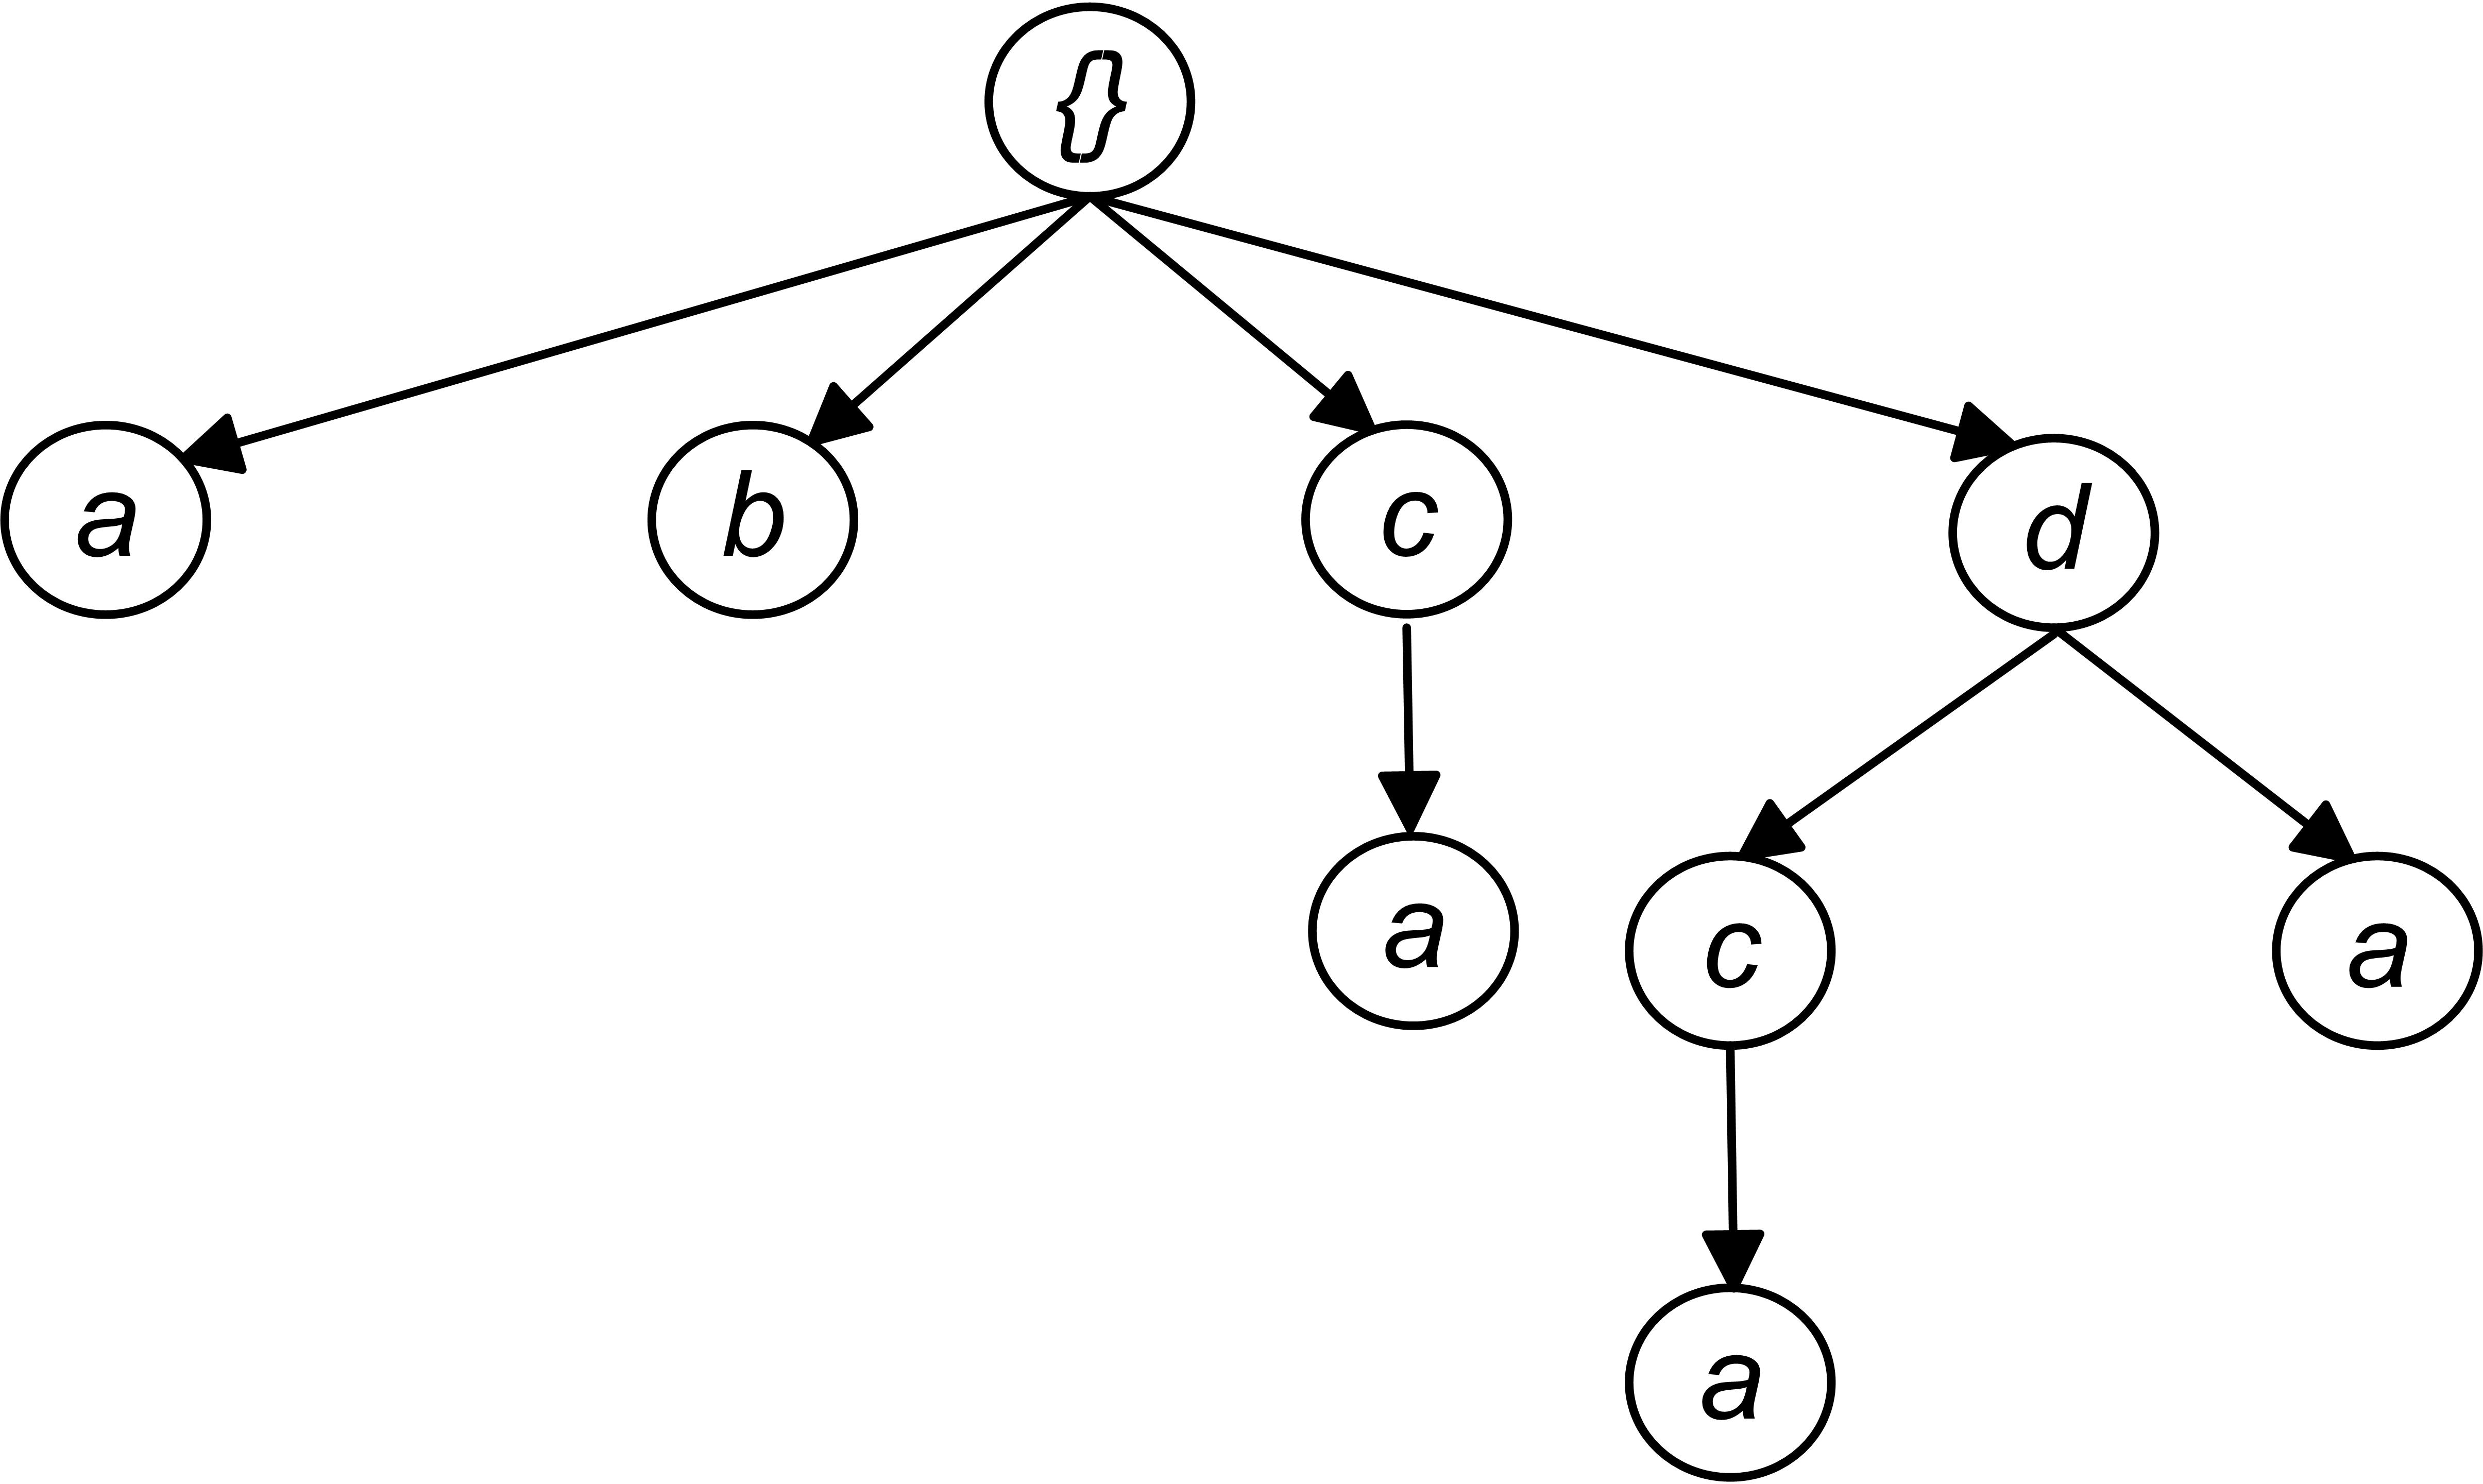
\includegraphics[width=\textwidth]{images/frequent_tree.jpg}
  \captionof{figure}{\emph{Frequent Item Tree} }
\end{minipage}
\caption{Frequent Patterns and Pattern Trees}
\label{figure:frequent_patterns}
\end{figure}
\begin{figure}
\begin{minipage}{.4\textwidth}
  \centering
  
	\begin{center}
	\begin{tabular}{ |c|c| } 
 	\hline
 		No & Items \\ \hline\hline
 		T\textsubscript{1} & \emph{a(0.9),c(0.6),d(0.5)}\\ \hline
 		T\textsubscript{2}& \emph{a(0.9),b(0.4),e(0.1)}\\ \hline
 		T\textsubscript{3}& \emph{a(0.2),c(0.9),d(0.7)}\\ \hline
 		T\textsubscript{4}& \emph{b(0.3),c(0.9)}\\ \hline
 		T\textsubscript{5}& \emph{a(0.1),b(0.3),c(0.9)} \\ \hline
 		T\textsubscript{6} & \emph{a(0.9),e(0.3)
}\\ \hline
\end{tabular}
\end{center}  
\end{minipage}
\hfill
\begin{minipage}{0.50\textwidth}
  \centering
  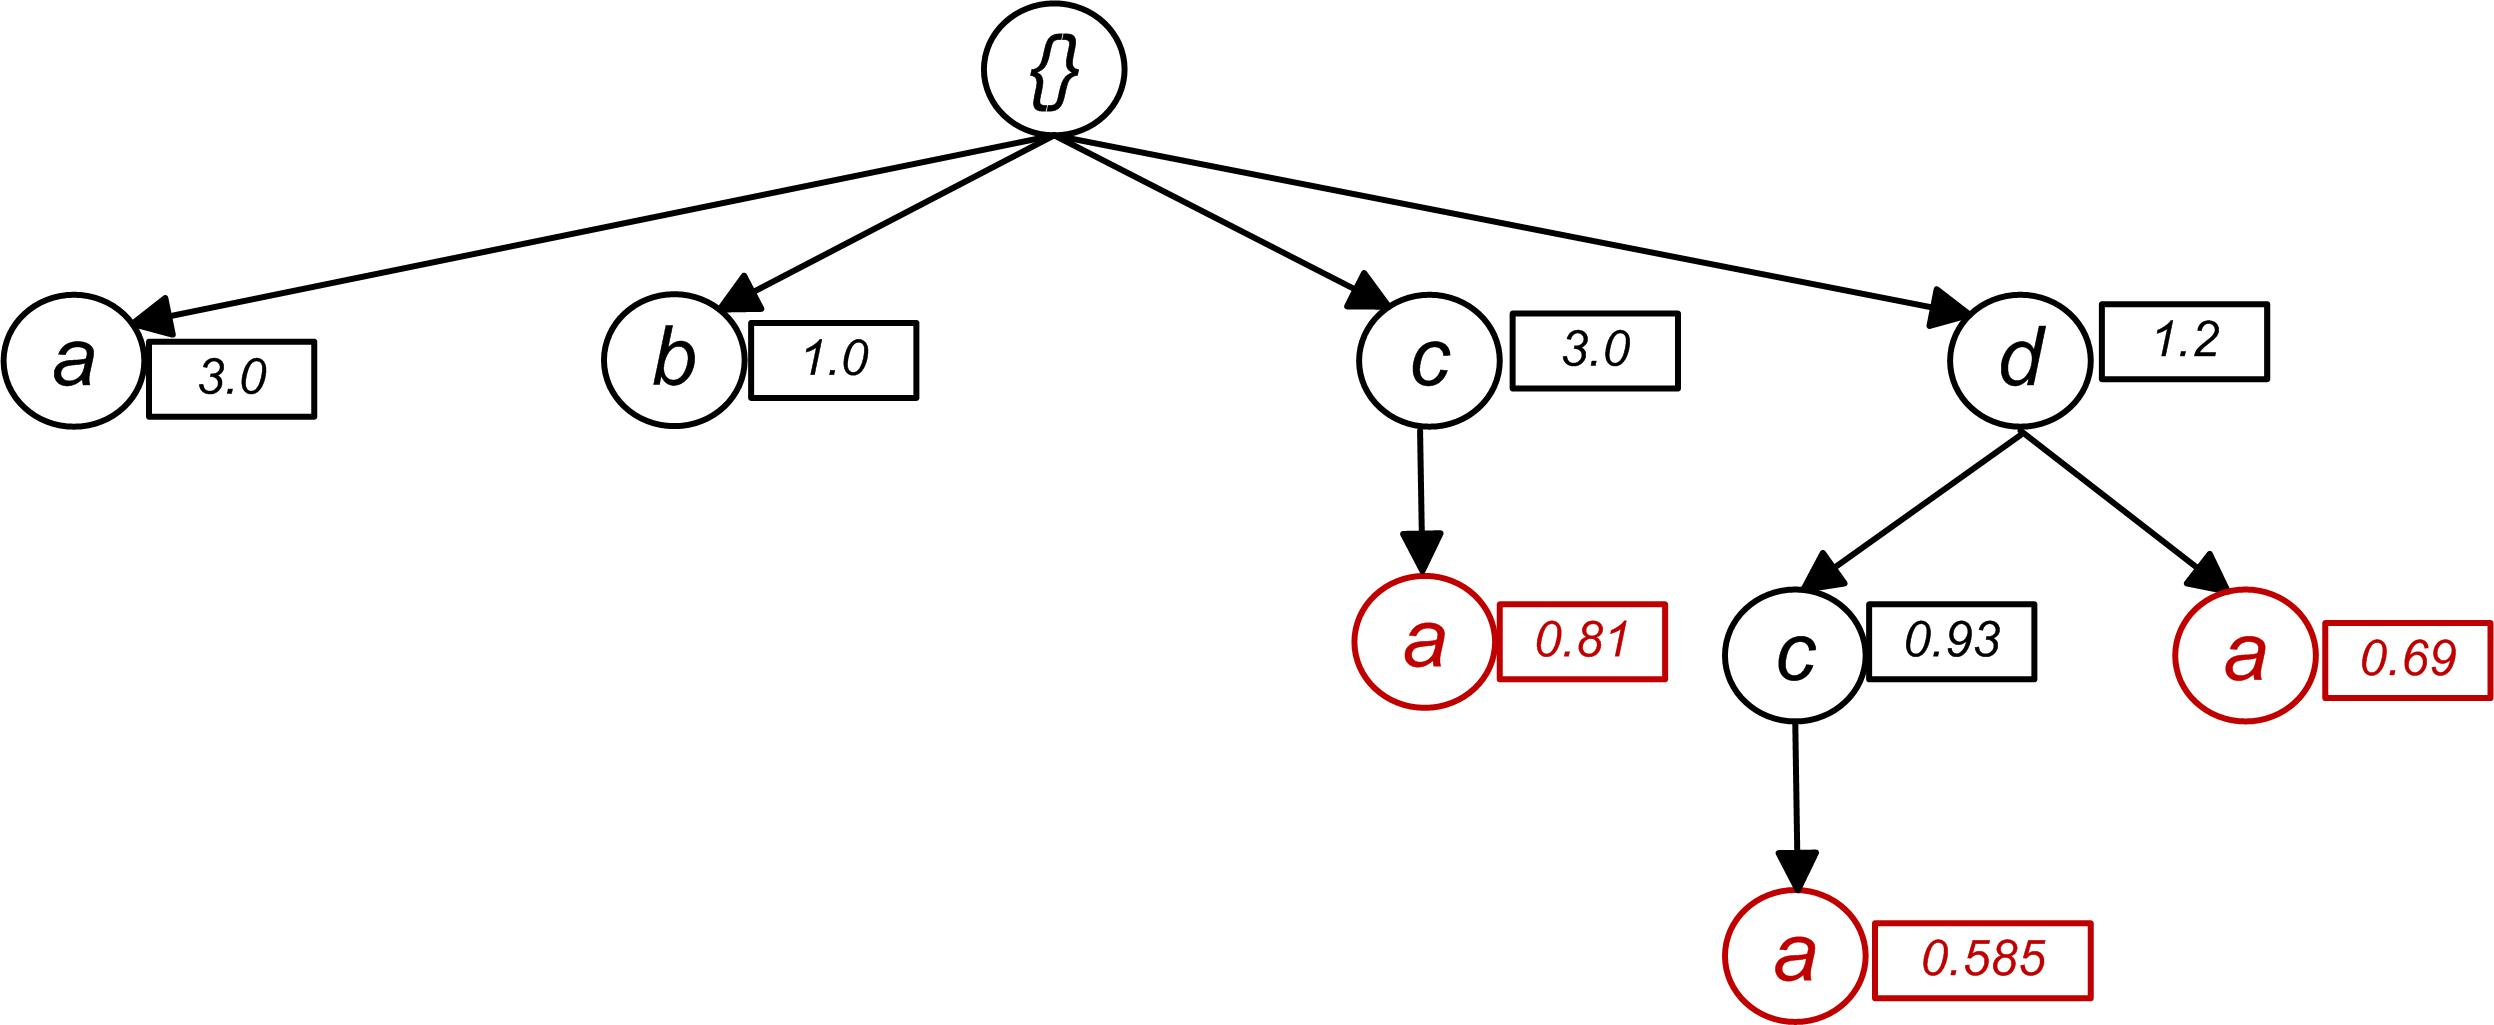
\includegraphics[width=\textwidth]{images/frequent_tree_final.jpg}
\end{minipage}
\caption{Transaction Table and Pattern Trees identifying \emph{False Positives}}
\label{figure:frequent_patterns_final}
\end{figure}
%\end{document}

%\end{document}